\documentclass[a4paper]{article}
\usepackage[utf8]{inputenc}
\usepackage[spanish, es-tabla, es-noshorthands]{babel}
\usepackage[table,xcdraw]{xcolor}
\usepackage[a4paper, footnotesep = 1cm, width=20cm, top=2.5cm, height=25cm, textwidth=18cm, textheight=25cm]{geometry}
%\geometry{showframe}

\usepackage{tikz}
\usepackage{amsmath}
\usepackage{amsfonts}
\usepackage{amssymb}
\usepackage{float}
\usepackage{graphicx}
\usepackage{caption}
\usepackage{subcaption}
\usepackage{multicol}
\usepackage{multirow}
\setlength{\doublerulesep}{\arrayrulewidth}
\usepackage{booktabs}

\usepackage{hyperref}
\hypersetup{
    colorlinks=true,
    linkcolor=blue,
    filecolor=magenta,      
    urlcolor=blue,
    citecolor=blue,    
}

\newcommand{\quotes}[1]{``#1''}
\usepackage{array}
\newcolumntype{C}[1]{>{\centering\let\newline\\\arraybackslash\hspace{0pt}}m{#1}}
\usepackage[american]{circuitikz}
\usetikzlibrary{calc}
\usepackage{fancyhdr}
\usepackage{units} 

\graphicspath{{../Calculos-Potencia/}{../Caracteristicas/}{../Consideraciones/}{../Gain-Stage/}{../Input-Stage/}{../Output-Stage/}{../Simulaciones/}{../Alimentacion/}{../Conclusiones/}}

\pagestyle{fancy}
\fancyhf{}
\lhead{22.12 Electrónica II}
\rhead{Mechoulam, Lambertucci, Rodriguez, Londero, Scala}
\rfoot{Página \thepage}

\begin{document}

En la siguiente sección, se busca elaborar una fuente regulada de tensión que cumpla con una salida que varíe entre $0 \ V$ y $9 \ V$, con una corriente de salida máxima de $2.5 \ A$. Dado que la tensión mínima debe ser nula, se implementó un regulador serie que utiliza un lazo de realimentación negativa que muestrea tensión y suma corriente, siendo así el circuito resultante el presentado a continuación.
\begin{figure}[H]
\centering
	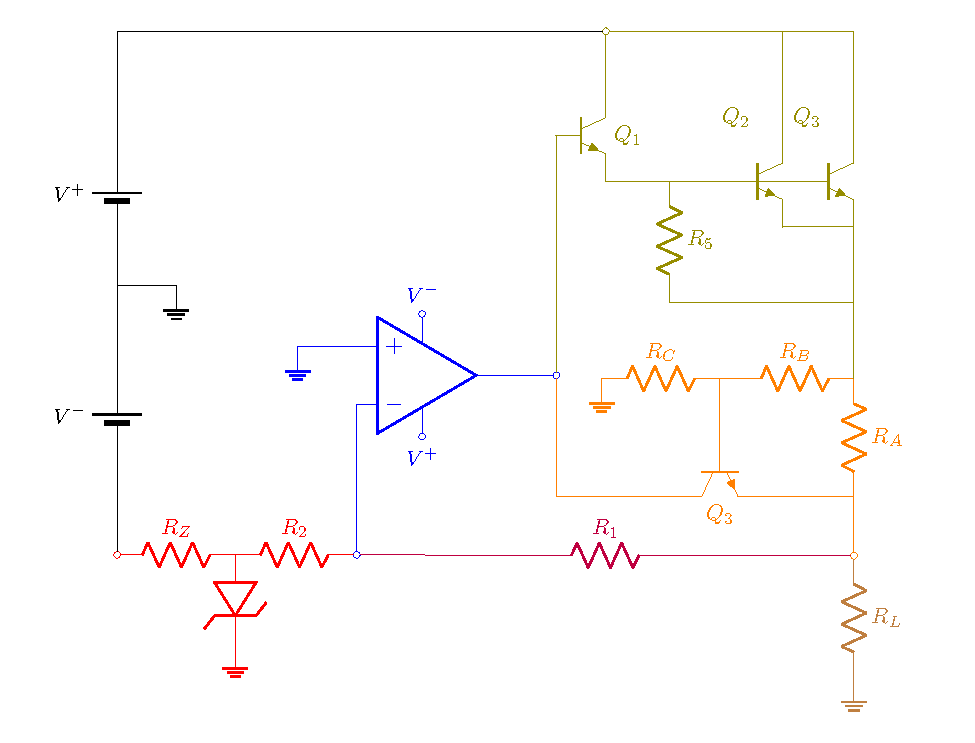
\includegraphics[width=1\textwidth, page=1]{ImagenesEjercicio2/Regulador.pdf}
	\caption{Circuito regulador de tensión.}
	\label{fig:circuito1}
\end{figure}

En la Figura (\ref{fig:circuito1}) se puede observar en distintos colores las diferentes etapas del sistema, siendo \textcolor{blue}{en azul el amplificador error}, \textcolor{orange}{en naranja el pre-regulador}, \textcolor{olive}{en verde el transistor de paso}, \textcolor{red}{en rojo el elemento de referencia}, \textcolor{purple}{en violeta el circuito de detección} y \textcolor{pink}{en rosado el circuito de protección}.

\begin{equation}
\frac{V^- - V_Z}{R_Z} + I_Z = \frac{V_Z}{R_9}
\end{equation}

\begin{equation}
V_{B1max} = V_{Oreg} + V_{Ra} + 1.4 \ V = 9 \ V + 1.25 \ V + 1.4 \ V = 11.65
\end{equation}

\begin{equation}
V_{2min} = 11.65 \ V + 1.5 \ V = 13.15 \ V
\end{equation}

\begin{equation}
	R_{Lmin} = \frac{V_{Omax}}{I_{Omax}} = 3.6 \ \Omega
\end{equation}

\begin{equation}
	R_{Lmax} = \infty
\end{equation}

\begin{equation}
	V_{Lmin} = R_Z \cdot \left( \frac{V_Z}{R_2} + I_z \right) + V_Z
\end{equation}

El pre-regulador cumple la función de brindar corriente \textbf{(habría que desarrollar un poco más)}. Para el caso presente, se observa que el amplificador operacional puede llegar hasta temperaturas de $125 \ ^o C$ son problema. Asumiendo una temperatura ambiente de $40 \ ^o C$, la potencia máxima disipada por operacional es de $0.7 \ W$.
\begin{figure}[H]
\centering
	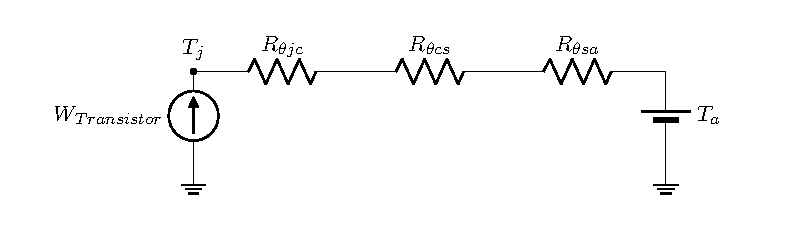
\includegraphics[width=0.6\textwidth, page=1]{ImagenesEjercicio2/Potencia.pdf}
	\caption{Circuito equivalente de potencias con $R_{\theta a-j} = 103 \ \frac{^o C}{W}$.}
	\label{fig:circuitopot}
\end{figure}

Es por ello que se analiza la potencia tanto en regulación como fuera de esta. Durante la primer etapa, la tensión de salida $V_O$ es estable pero la corriente es cada vez mayor. A pesar de esto, la potencia disipada por el opamp se mantiene menor a la máxima. Por otro lado, con el circuito fodlback activado, la tensión decae, haciendo que también decaiga la potencia del amplificador, manteniendola por debajo del máximo.
\begin{figure}[H]
\centering
	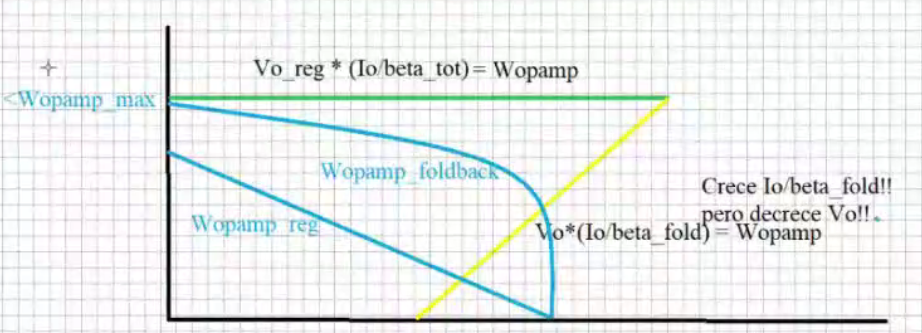
\includegraphics[width=0.6\textwidth]{ImagenesEjercicio2/Potencia2.png}
	\caption{Curvas de potencia consumida.}
	\label{fig:curvapot}
\end{figure}


\end{document}